\documentclass[11pt]{a0poster}

\usepackage{url}
\usepackage{graphicx}
\usepackage[usenames,dvipsnames]{color}
\usepackage[margin=0in]{geometry}
\usepackage{xcolor}
\usepackage{graphicx}
\usepackage{amsmath}

\widowpenalty=500
\clubpenalty=500
\fboxsep=0pt

\renewcommand*{\familydefault}{\sfdefault}

\date{}

\begin{document}

\begin{minipage}{0.887\linewidth}
\vspace{100pt}
\hspace{100pt}
\color{Blue}
{\fontsize{3cm}{1em} \bf avocado: A Variant Caller, Distributed}

\hspace{100pt}
\huge Frank Austin Nothaft, Peter Jin, Brielin Brown

\hspace{100pt}
\huge \{fnothaft, phj, brielin\}@berkeley.edu
\vspace{100pt}
\end{minipage}
\begin{minipage}{0.113\linewidth}

\includegraphics[scale=0.6]{ucseal_540_139.pdf}
\end{minipage}

{\color{Blue}\noindent\makebox[\linewidth]{\rule{\paperwidth}{30pt}}}

\noindent\colorbox{Yellow}{
\begin{minipage}[t][2045pt][t]{\linewidth}

\noindent\begin{minipage}{0.025\linewidth}
\hfill
\pagebreak
\end{minipage}
\begin{minipage}{0.3\linewidth}
\vspace{75pt}
\colorbox{Blue}{
\begin{minipage}{\linewidth}
\vspace{25pt}
\begin{center}
\Huge \bf \color{White} Background
\end{center}
\vspace{10pt}
\end{minipage}
}
\colorbox{White}{
\begin{minipage}[t][600pt][t]{\linewidth}
\color{Blue}
\vspace{20pt}
\LARGE Three stages in modern DNA processing pipelines:
\begin{enumerate}
\item {\bf Sequencing:} Generate 100-250 base pair reads
\item {\bf Alignment:} Align these reads to the reference genome
\item {\bf Variant Calling:} Determine gene variants \& genotypes
\end{enumerate}
Variant calling is an interesting area: ``Accurate'' algorithms are slow and don't
scale (60 hrs/genome), and are inaccurate for high complexity regions (error is $>75\%$).

\textbf{Goals:}
\begin{enumerate}
\item Build a variant caller designed for distributed computing
\item Develop an open-source alternative to the GATK
\end{enumerate}
\hfill
\pagebreak
\end{minipage}
}

\vspace{75pt}
\colorbox{Blue}{
\begin{minipage}{\linewidth}
\vspace{25pt}
\begin{center}
\Huge \bf \color{White} Pipeline
\end{center}
\vspace{10pt}
\end{minipage}
}
\colorbox{White}{
\begin{minipage}[t][1020pt][t]{\linewidth}
\color{Blue}
\vspace{20pt}
\LARGE
\textbf{Tech Specs:}
\begin{itemize}
\item Built in Scala on top of Parquet and BDAS Spark
\item Leverages new ADAM read/pileup/variant call format
\item Scalability well past 30+ nodes; other pipelines are limited to 26 (1/chromosome)
\end{itemize}
\textbf{Pipeline:} \\
\begin{center}
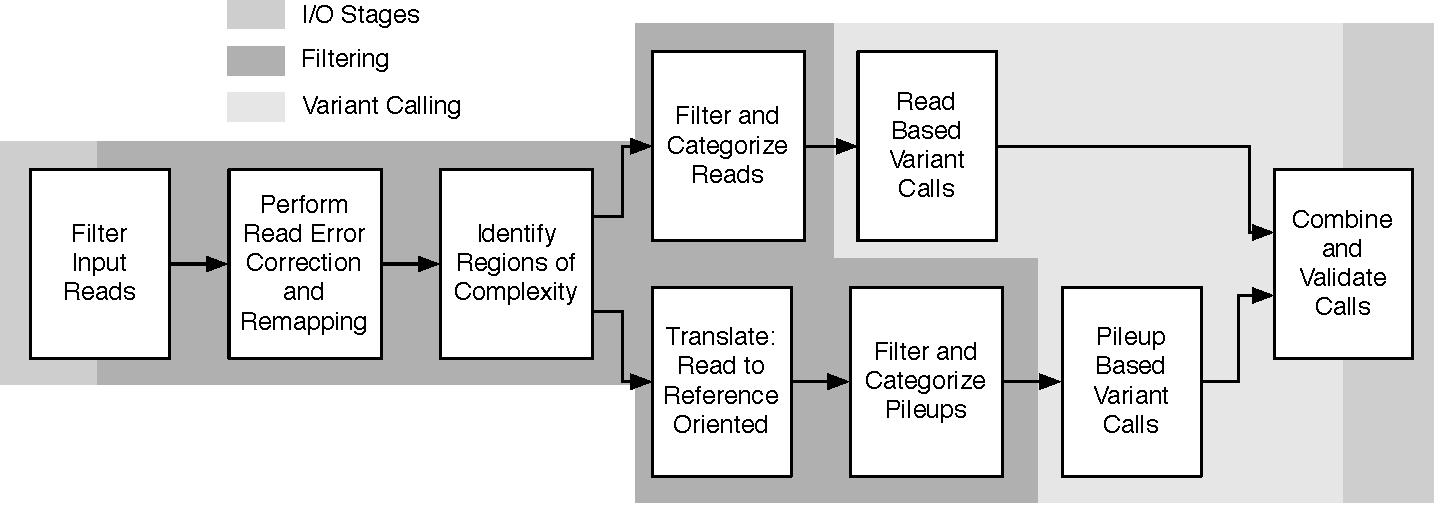
\includegraphics[width=0.9\linewidth]{avocado-architecture.pdf}
\end{center} 
\textbf{Design Principles:}
\begin{itemize}
\item Reuse read processing stages from ADAM
\item Use mapping quality/coverage as filtering heuristic
\item Design is modular: easy to add new calling algorithms
\end{itemize}
\pagebreak
\end{minipage}
}
\pagebreak
\end{minipage}
\begin{minipage}{0.03\linewidth}
\hfill
\pagebreak
\end{minipage}
\begin{minipage}{0.6\linewidth}

\vspace{70pt}
\colorbox{Blue}{
\begin{minipage}[t]{\linewidth}
\vspace{30pt}
\begin{center}
\Huge \bf \color{White} Performance
\end{center}
\vspace{17pt}
\end{minipage}
}
\colorbox{White}{
\begin{minipage}[t][500pt][t]{\linewidth}
\hfill
\pagebreak
\end{minipage}
}

\vspace{75pt}
\colorbox{Blue}{
\begin{minipage}[t]{\linewidth}
\vspace{30pt}
\begin{center}
\Huge \bf \color{White} Local Assembly
\end{center}
\vspace{17pt}
\end{minipage}
}
\colorbox{White}{
\begin{minipage}[t][400pt][t]{0.3\linewidth}
\vspace{20pt}
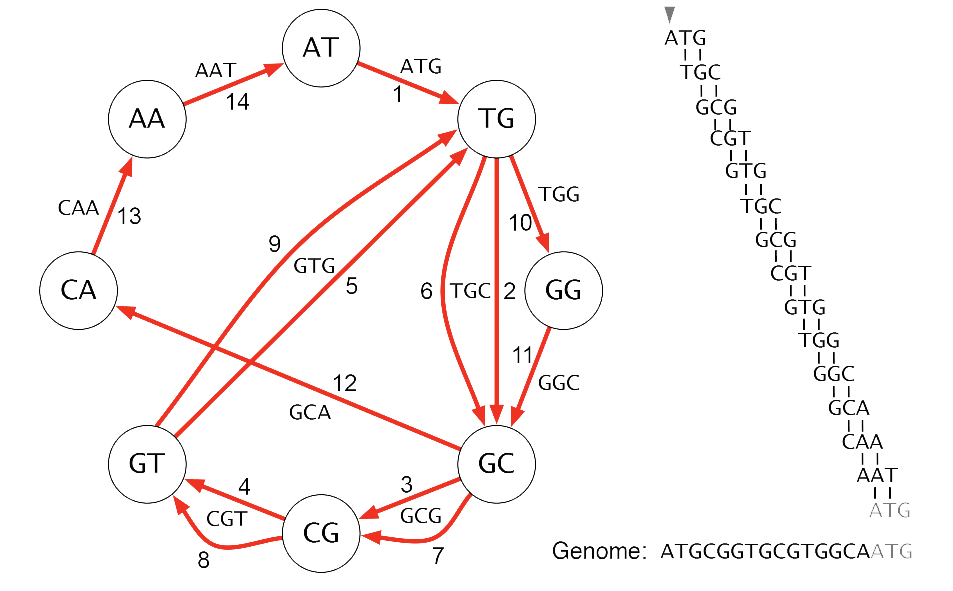
\includegraphics[width=0.9\linewidth]{assembly-fig.pdf}
\pagebreak
\end{minipage}
\begin{minipage}[t][400pt][t]{0.7\linewidth}
\vspace{20pt}
\LARGE We partition the high-complexity locations into regions and use local
$k$-mer assembly to discover the most likely haplotype pair per region.
%The $k$-mer assembly slices the reads in a region into $k$-mer edges (i.e.,
%strings of length $k$), and the overlaps between edges form the $k$-mer graph.
The likelihood of a pair of haplotypes $H_j$ and $H_{j'}$ is given by:
\large $$ \mathcal{L}(H_j,H_{j'})=\prod_i\left[ \frac{P(r_i|H_j)}{2}+\frac{P(r_i|H_{j'})}{2} \right] $$
\LARGE where $r_i$ is a read.
We obtain $P(r|H)$ by a pairwise HMM alignment model.

\small \hfill

\small Figure credit:
  P.E.C.~Compeau, P.A.~Pevner, G.~Tesler,
  ``How to apply de Bruijn graphs to genome assembly,'' Nature Biotech.~29(11), 2011.
\pagebreak
\end{minipage}
}

\vspace{75pt}
\begin{minipage}{0.47\linewidth}
\colorbox{Blue}{
\begin{minipage}[t]{\linewidth}
\vspace{30pt}
\begin{center}
\Huge \bf \color{White} Base SNP Calling
\end{center}
\vspace{17pt}
\end{minipage}
}
\colorbox{White}{
\begin{minipage}[t][520pt][t]{\linewidth}
\color{Blue}
\vspace{20pt}
\LARGE For calling SNPs on a single sample, we look at genome loci that show evidence
of a SNP (at least one non-reference base). Genotype likelihoods are calculated
by:
\large$$\mathcal{L}(g)=\frac{1}{m^k}\prod_{j=1}^{l}{(m - g) \epsilon + g (1 - \epsilon)}\prod_{j=l + 1}^{k}{(m - g)(1 - \epsilon) + g \epsilon}$$
\begin{center}
\small $m$ = ploidy, $g$ = genotype state, $\epsilon$ = likelihood of error, \\
$l$ = bases matching reference, $k$ = bases at locus
\end{center}
\LARGE Genotyping is biased towards the reference. We compensate by the allele
frequency and call a non-reference genotype if $g \in (1, 2)$ has the highest probability.
\pagebreak
\end{minipage}
}
\end{minipage}
\begin{minipage}{0.06\linewidth}
\hfill
\pagebreak
\end{minipage}
\begin{minipage}{0.47\linewidth}
\colorbox{Blue}{
\begin{minipage}[t]{\linewidth}
\vspace{30pt}
\begin{center}
\Huge \bf \color{White} Sufficient Statistics/Joint Calling
\end{center}
\vspace{17pt}
\end{minipage}
}
\colorbox{White}{
\begin{minipage}[t][520pt][t]{\linewidth}
\color{Blue}
\vspace{20pt}
\LARGE For a few samples, one may look-up the MAF $\phi$ in a reference and compensate the
the single sample likelihood
\large $$\hat{g} = \arg\max_{g} \mathcal{L}(g)\mathbf{P}(g | \phi)$$ 
\LARGE When many samples are collected it can be desirable to compute a population MAF while
performing genotype calling. For each SNP $a$, this is done via EM:

\large $$ \phi_{a,t+1} = \frac{1}{M}\sum_{i=1}^N \frac{\sum_{g_i} g_i  \mathcal{L}(g_i)\mathbf{P}(g_i | \phi_{a,t}) }{ \sum_{g_i} \mathcal{L}(g)\mathbf{P}(g | \phi_{a,t})} $$
\begin{center}
$M = \sum_i m_i$ = total number of chromosomes $N$ = number of individuals
\end{center}
\pagebreak
\end{minipage}
}
\end{minipage}

\pagebreak
\end{minipage}
\end{minipage}
}

\end{document}
